\addtocontents{toc}{\protect\vspace{\beforebibskip}} % Place slightly below the rest of the document content in the table

%************************************************
\chapter{Kensentme Platform Delevopment}
\label{ch:development}
%************************************************

The internship started on September 2nd 2019, being planned to last for 9 months, ending on the 29th of May 2020.

The main goal of the internship is the development of a collaborative platform based on Autopsy, which was soon named ``Kensentme`` by the company's designer.

Each step taken towards the development of this platform is documented in this chapter, from project planning to full roll out on a production environment.

\section{Development Framework}

The project development followed an agile workflow, using a JIRA board to organize bi-weekly sprints.

The project had four intervinient parties involved. The developer was responsible for developing the software. The product owner provided help in decisions surrounding the developed product. 
The designer came up with ideas for the user interface and user experience of the platform. And the tester made sure everything was working as intended.

For each sprint the process was identical, a sprint review was conducted to assess the progress made in the previous sprint, then a new sprint would be planned by the developer, 
the features would be implemented during the two week duration of the sprint, and developed features would be tested thoroughly before the sprint ended.

\section{Project Planning}

Autopsy by itself is capable of providing a distributed solution for multi user collaboration, but it is very resource intensive and requires many complex configuration steps,
and is also only fully supported on the Windows O.S.

The plan for this internship is to achieve the same kind of functionality provided by the original software, but without the dependency on harduous pre-configuration
or hardware intensive requirements, resulting in needing only single capable server, and allowing the program to be used by multiple low capacity client devices using 
any web capable O.S.

To achieve that goal, the project will be an adaptation of the original Autopsy source code, into a client-server model, with the server developed in Java using the Quarkus \cite{quarkus} framework,
and the client developed in Javascript using the React \cite{react} framework.

The project is outlined to work in a multi user environment, allowing users to be assigned to teams and teams assigned to cases, and allowing multiple users to interact with
a case simultaneously.

Autopsy has a major limitation, which is it only allows one case to be open at a time, ideally in this project we should find a workarround to allow working on multiple cases
at once, but we feel like dedicating a server instance (which a single machine can have many virtualized within) per case is a good enough approach, though as future work the
ability to spawn different containers as requested to work on different cases at once is an interesting challenge.

Given that the core features will be running in a remote server, it was decided that the addition of data sources to cases will be handled by an FTP client, allowing users
to transfer files to their respective data source directories, and FTP access will be controlled according to each user's credentials on the platform.

The architecture of the expected result is represented in Figure \ref{fig:arch}, where it can be seen that multiple clients can connect through REST API, WebSockets and FTP with the Kensentme server, 
which requests and provides data to both database and indexation servers.

\begin{figure}[ht]
 \centering
 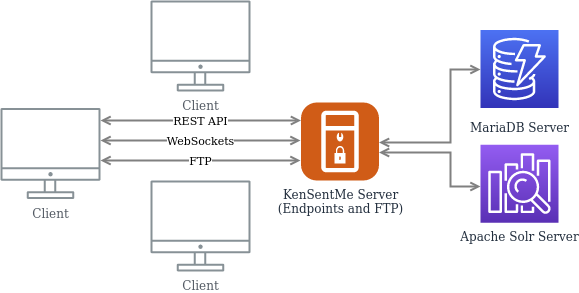
\includegraphics[width=0.75\linewidth]{imgs/arch.png}
 \caption{Software Arquitecture}
 \label{fig:arch}
\end{figure}


\section{Autopsy Source Code Analysis}

Autopsy is a digital forensics analysis software that is available as Open Source Software \cite{opensource} on \citetitle{github} \cite{github}.

With the goals set for this project, the source code was analyzed to understand which components need to be replicated and adapted in order to obtain the same logic flow.

The ``Core`` module is where the most important components are located, and after analysis it was concluded that the following directories contain relevant information, as can be seen in Table \ref{tab:autopsyOverview}.

\begin{tabularx}{\textwidth}{@{}|c| *1{>{\centering\arraybackslash}X}@{}|}
    \hline
    \textbf{Name} & \textbf{Description} \\
    \hline\hline
    Actions & user interactions  \\
    \hline
    Casemodule & case class and other resources needed for the functioning of an autopsy case like data sources and artifacts \\
    \hline
    Centralrepository & data persisted and accessed by multiple cases (Correlation Engine) \\
    \hline
    Contentviewers & panels used for data representation  \\
    \hline
    Coordinationservice & configuration information distribution system \\
    \hline
    Core & addition of command line options, system configurations and collaboration monitor  \\
    \hline
    Corecomponents & main user interface components \\
    \hline
    Datamodel & all the entities needed to represent ingested data \\
    \hline
    Datasourceprocessors & data processing utilities  \\
    \hline
    Directorytree & file explorer for ingested artifacts \\
    \hline
    Ingest & utilities and events for data ingestion  \\
    \hline
    Keywordsearchservice & utility to search artifacts by keyword  \\
    \hline
    Modules & all the pre-included modules (data ingestion procedures) \\
    \hline
    Progress & progress indicators and similar classes \\
    \hline
    Python & resources needed for the functioning of the Jython language \\
    \hline
    Rejview & resources used to analyse Windows registry \\
    \hline
    Report & report generation utilities and modules \\
    \hline
    Timeline & recent addition to Autopsy, allows visualization of artifacts in temporal chart, only available for Windows O.S. \\
    \hline
    \caption{Autopsy Modules Overview}
    \label{tab:autopsyOverview}
\end{tabularx}


The ``KeywordSearch`` module is also of critical importance as it provides one of the most meaningful features which is filtering all the artifacts in a case with a keyword
search using the Apache Solr search platform, which indexes the text contents of all the artifacts and allows extremely fast searching through a large amount of data.  

Another module that needs to be adapted is the ``RecentActivity`` module, which contains the tools needed to extract information from browsers, registry and other important resources, providing a great amount of
critical evidence from data sources.

Each autopsy case contains it's own SQLite database, which contains the tables present in Table \ref{tab:tables}.

\begin{tabularx}{\textwidth}{|c|c|c|}
    \hline
    tsk\_db\_info & tsk\_db\_info\_extended & tsk\_objects \\
    \hline
    tsk\_image\_info & tsk\_image\_names & tsk\_vs\_info \\
    \hline
    tsk\_vs\_parts & tsk\_fs\_info & data\_source\_info \\
    \hline
    tsk\_files & file\_encoding\_types & tsk\_files\_path \\
    \hline
    tsk\_files\_derived & tsk\_files\_derived\_method & tag\_names \\
    \hline
    review\_statuses & blackboard\_artifacts & blackboard\_attributes \\
    \hline
    ingest\_modules & blackboard\_attribute\_types & ingest\_module\_types \\
    \hline
    reports & blackboard\_artifact\_types & ingest\_jobs \\
    \hline
    ingest\_job\_modules & ingest\_job\_status\_types & account\_types \\
    \hline
    accounts & account\_relationships & tsk\_event\_types \\
    \hline
    tsk\_examiners & blackboard\_artifact\_tags & content\_tags \\
    \hline
    tsk\_file\_layout & tsk\_event\_descriptions & tsk\_events \\
    \hline
    tsk\_pool\_info & & \\
    \hline
    \caption{Case Database Tables}
    \label{tab:tables}
\end{tabularx}

The tables containing the information accessed most frequently are the ones related to blackboard artifacts, along with tables related to files and tags.

Autopsy's source code allows access to most of the important entities present in this database, through pre-defined queries which return entities like data sources, abstract files, or artifacts. 
But in order to add features like pagination and tag deletion, custom queries must be created, so that the queries may return only a specific amount of entity ids, or so that delete commands may be executed. 

\section{Development Stages}

\subsection{Basic Autopsy Functionalities}

As a first step into replicating the functionalities of the original program, the most basic functionality from Autopsy was adapted, the ability to open an Autopsy case. For this some elements of the original Casemodule package were adapted,
and after that all the other similar actions like closing, creating and deleting cases were also adapted.

Autopsy cases have a case file containing case metadata, which allows the program to connect to the right database when the case is open, this database is also present
in a file inside the filesystem, which uses the SQLite database engine, so for the cases to be usable in the server these files must also be present in the server,
which resulted in the creation of a directory within the server called ``repository``, containing all the different cases created within the application.

Later in the development there was the need to create an additional directory alongside the ``repository`` called ``central-repository``
which contains the database used by the Correlation Engine, which is a feature that finds files present in multiple cases, to ingest data that can be queried by any case.

The development of autopsy features was done alongside the original software, so that every new feature implemented into the platform could be compared and verified with the original software, and it was reassuring to see that cases created 
through one of the versions of the software were capable of being opened through the other version, meaning that the source code provided by autopsy, with some tinkering, can definetely be used in a client-server model.

\subsection{Authentication Process}

The authentication process is handled through a REST API, when the authentication is completed the user receives a JSON Web Token (JWT).

JWT is an open standard that defines a compact and self-contained way for securely transmitting information between parties. This information can be verified and trusted because it is digitally signed.
JWT contain three parts, as can be seen in Table \ref{tab:jwtComposition}.

\begin{table}[ht]
  \begin{tabularx}{\textwidth}{@{}|c| *1{>{\centering\arraybackslash}X}@{}|}
    \hline
    \textbf{Name} & \textbf{Contents} \\
    \hline\hline
    Header & Information about the signing algorithm used  \\
    \hline
    Payload & Information about the user, such as username, e-mail and roles \\
    \hline
    Signature & A signature used to verify the contents weren't changed \\
    \hline
  \end{tabularx}
  \caption{JWT Composition}
  \label{tab:jwtComposition}
\end{table}

The authentication can be performed with either username or e-mail and a password, and extra authentication factors can be added such as One Time Passwords (OTP) and Universal Second Factor (U2F).

If no extra factors were added to an account, the authentication attempt with the user's credentials will return the JWT when successful and the user can freely access protected content.

When extra factors are present in an account, the response from the same request will contain an array with the extra factors added, and a UUID, which is a pseudo random string, which must be sent in the next request to validate the user's identity.
This UUID is saved in the database in the form of salted hash using the blowfish algorithm, and is invalidated after a successful login attempt. The user then has the choice between any of the extra factors and must complete the required steps to validate that factor, as can be seen in Figure \ref{fig:login}.

\begin{figure}[ht]
 \centering
 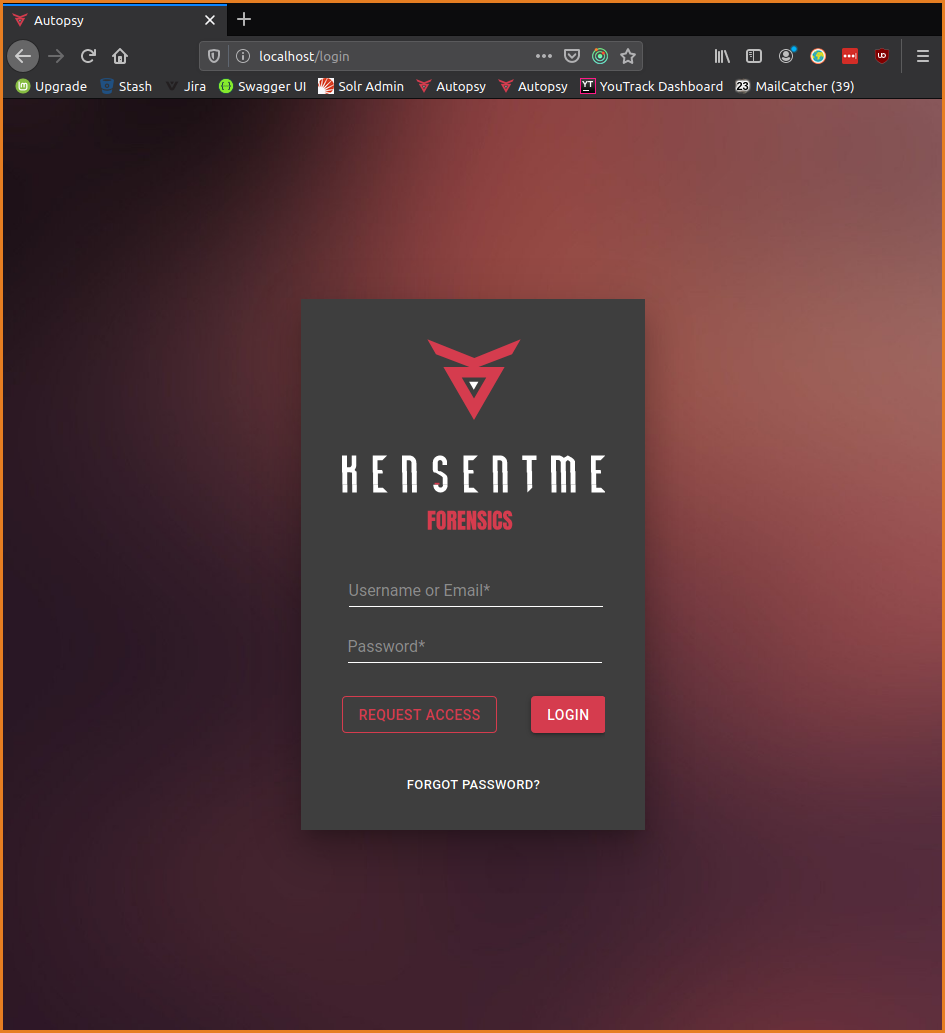
\includegraphics[width=0.35\linewidth]{imgs/login.png}
 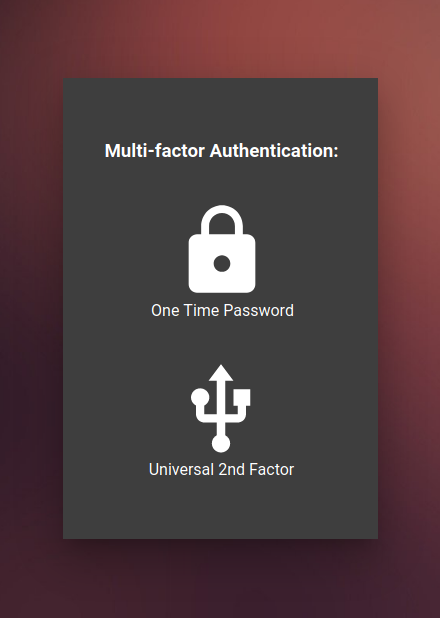
\includegraphics[width=0.35\linewidth]{imgs/mfa.png}
 \caption{Login Screen and Extra Factors}
 \label{fig:login}
\end{figure}

\subsubsection*{One Time Password}

The process of seting up OTP for an account begins with generating a secret string, which is used by both the server and the authenticator app to generate OTP, when the secret is generated, it is saved as a temporary secret after being encrypted by the RSA algorithm.

The temporary secret must be added to the user's device, either by inserting the string itself or by scanning a QR code, and must be validated by the user by submitting the current OTP, after validation the temporary secret is considered permanent.

All OTP validations have a 30 second threshold, which means the current OTP is valid for an extra 30 seconds after being replaced by the next OTP, allowing the user to have a better experience with these passwords.

The processes of authenticating and removing this authentication factor both depend on validating the current OTP, which is provided by the user's app.

In the event of loss of the device that the user uses to generate OTP, all the authentication factors can be reset using the ''Reset Password'' functionality, which relies on e-mail validation to prove the user's identity.

\subsubsection*{Universal Second Factor}

TODO

\subsection{Management Entities}

As a first step in the development, the different persisted entities were created, which are Users, Teams, and Cases. All the endpoints for actions involving these 
entities were created, resulting in the ability for the client program to interact with these entities and modify their relationships and other variables.
For these functionalities there are two roles associated, the Manager role allows manipulation of the existing entities while the Investigator role only has access to his
own information and the teams and cases he was assigned to. For these interactions, it was decided to create a drag and drop interface, which allows users to be dragged into
teams and teams dragged into cases. All these entities are listed side by side and each have their own options and filtering input, as can be observed in Figure \ref{fig:users}.

\begin{figure}[ht]
 \centering
 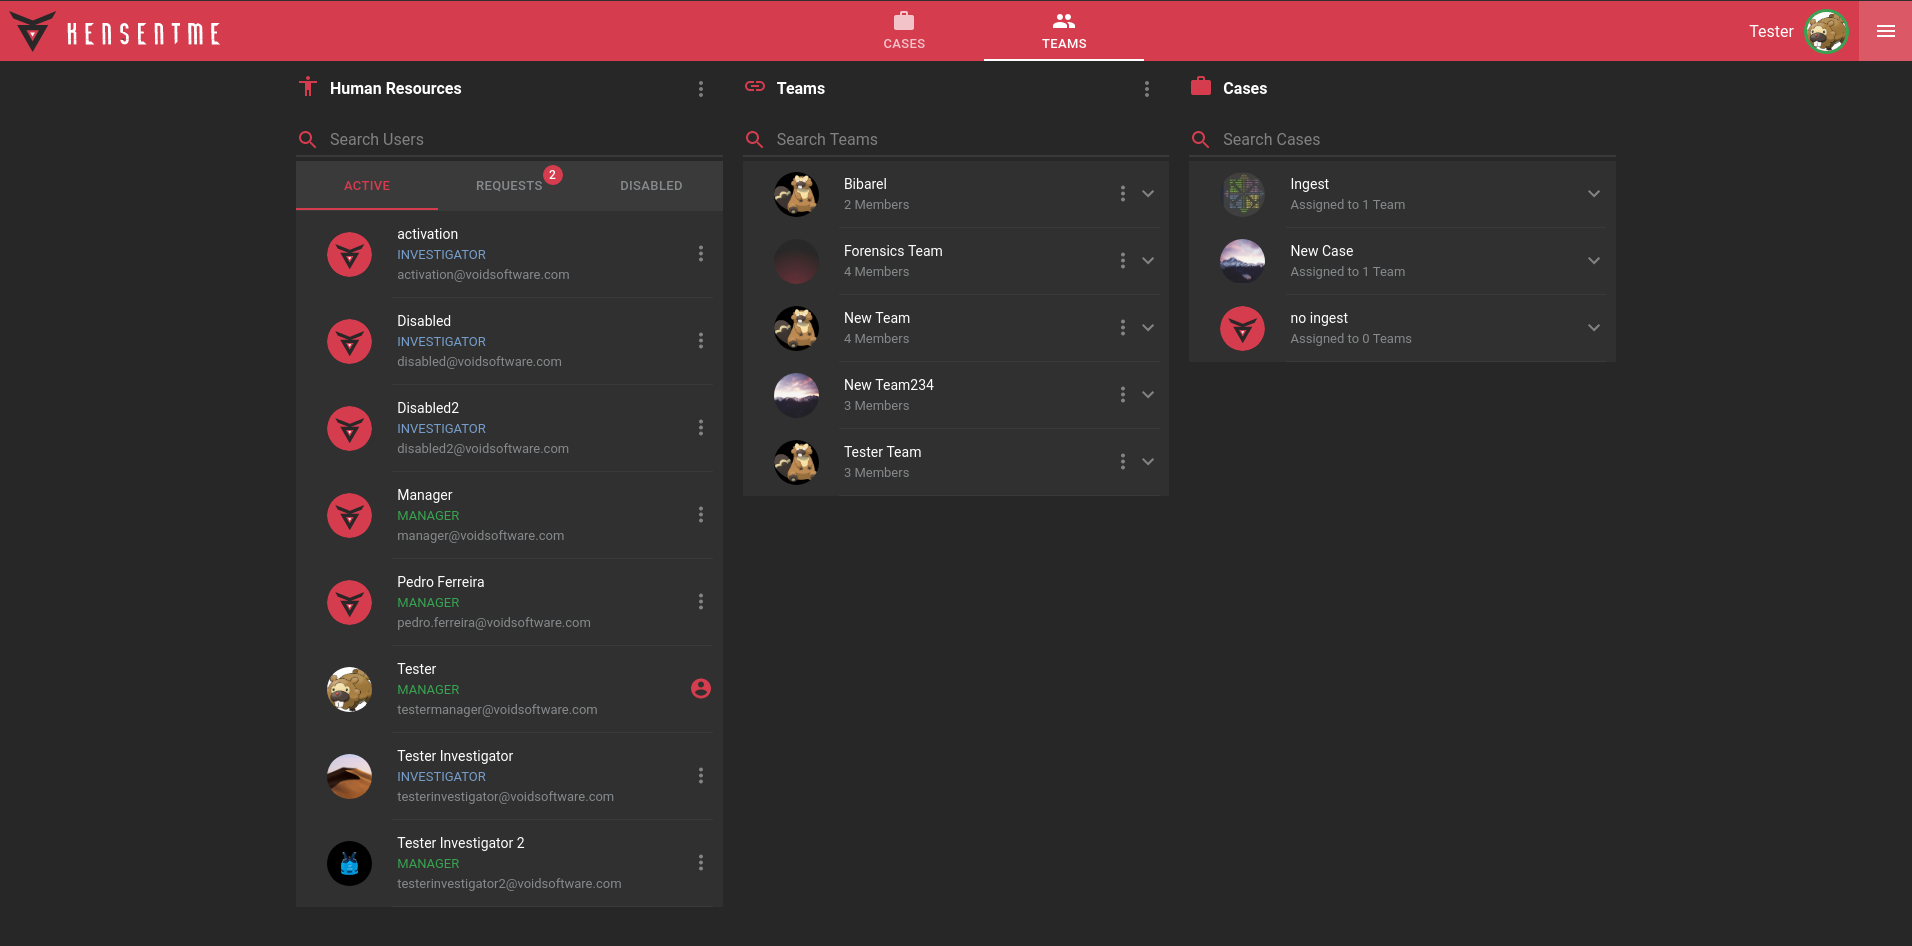
\includegraphics[width=1\linewidth]{imgs/users.png}
 \caption{Entity Management Interface}
 \label{fig:users}
\end{figure}

Users can change their own profile picture, while Managers can also change any team or case's display picture.
Managers can add new users to the platform, can approve membership requests, can enable/disable user accounts and can create new teams.
When a user is added by a Manager or his membership request is approved, he must define a password when activating his account through a received e-mail message.

It was at this step in development that was made clear by the testers, that validations must be preformed on both server and client side, and that error handling must be streamlined
in order to provide a seemless experience to the user, while also allowing future additions to the platform to be implemented in a similar way without much tinkering. Because even though 
the platform still wasn't fully developed, it already suffered from possible exploits that could break the experience for it's users, like the upload of a 5GB file as an image file, which would stop the page from loading, 
or possible directory traversal attacks, resulting from the creation of case directories.

The lessons learned from the testers on this stage of development carried on through the entire development process and ensured that every new feature added was accounting for possible weaknesses which may result from the new 
implementations, resulting in a more secure development process.

The platform's resulting data model can be observed in Figure \ref{fig:database}.

\begin{figure}[ht]
 \centering
 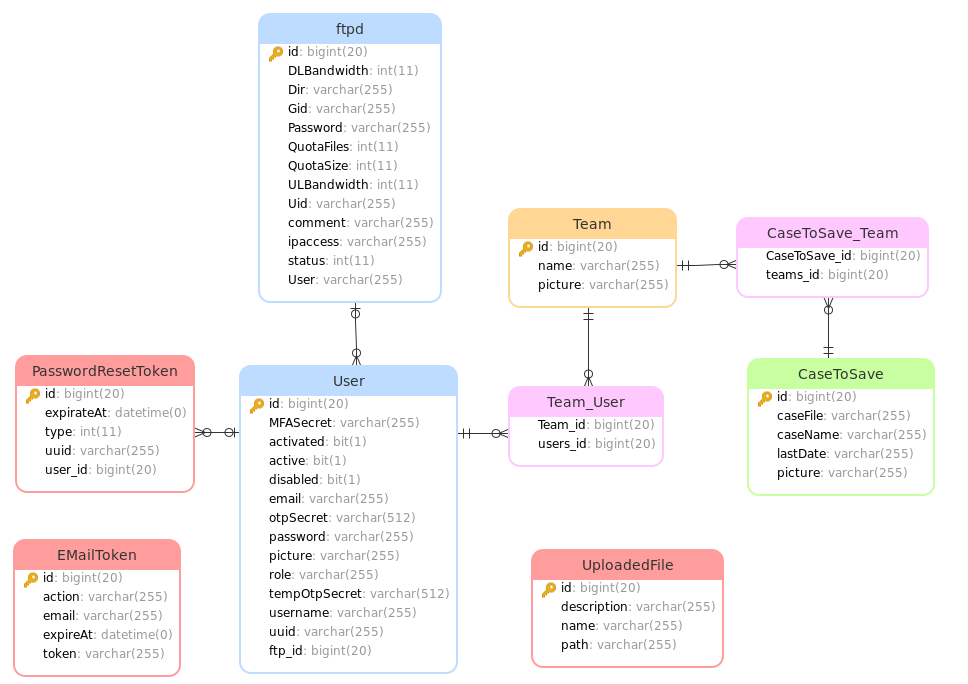
\includegraphics[width=1\linewidth]{imgs/database.png}
 \caption{Database Structure}
 \label{fig:database}
\end{figure}

\subsection{Ingested Results Presentation}

Ingested results are the items present inside the provided data sources, Autopsy can run multiple modules on each data source to extract results, and the extracted results can either be a file instance or an artifact instance.
The difference between a file and an artifact is that an artifact represents only a smaller piece of a file's information, which means a file can contain multiple artifacts, for example a registry file can contain multiple O.S. user account artifacts.

Even though the data ingestion features weren't implemented yet on the platform, the data that was ingested into a case using the original program could also be used on this platform, which allowed this feature to be developed earlier.

The ingested results are presented in three different containers, one taking the shape of a file explorer, allowing exploration of the structure of all the results, 
one taking the shape of a table or thumbnail viewer, presenting all the contents of the results selected from the explorer, and one taking the shape of a content viewer, allowing visualization
of the data contained inside the result selected from the table as can be seen in Figure \ref{fig:data}.

\begin{figure}[ht]
 \centering
 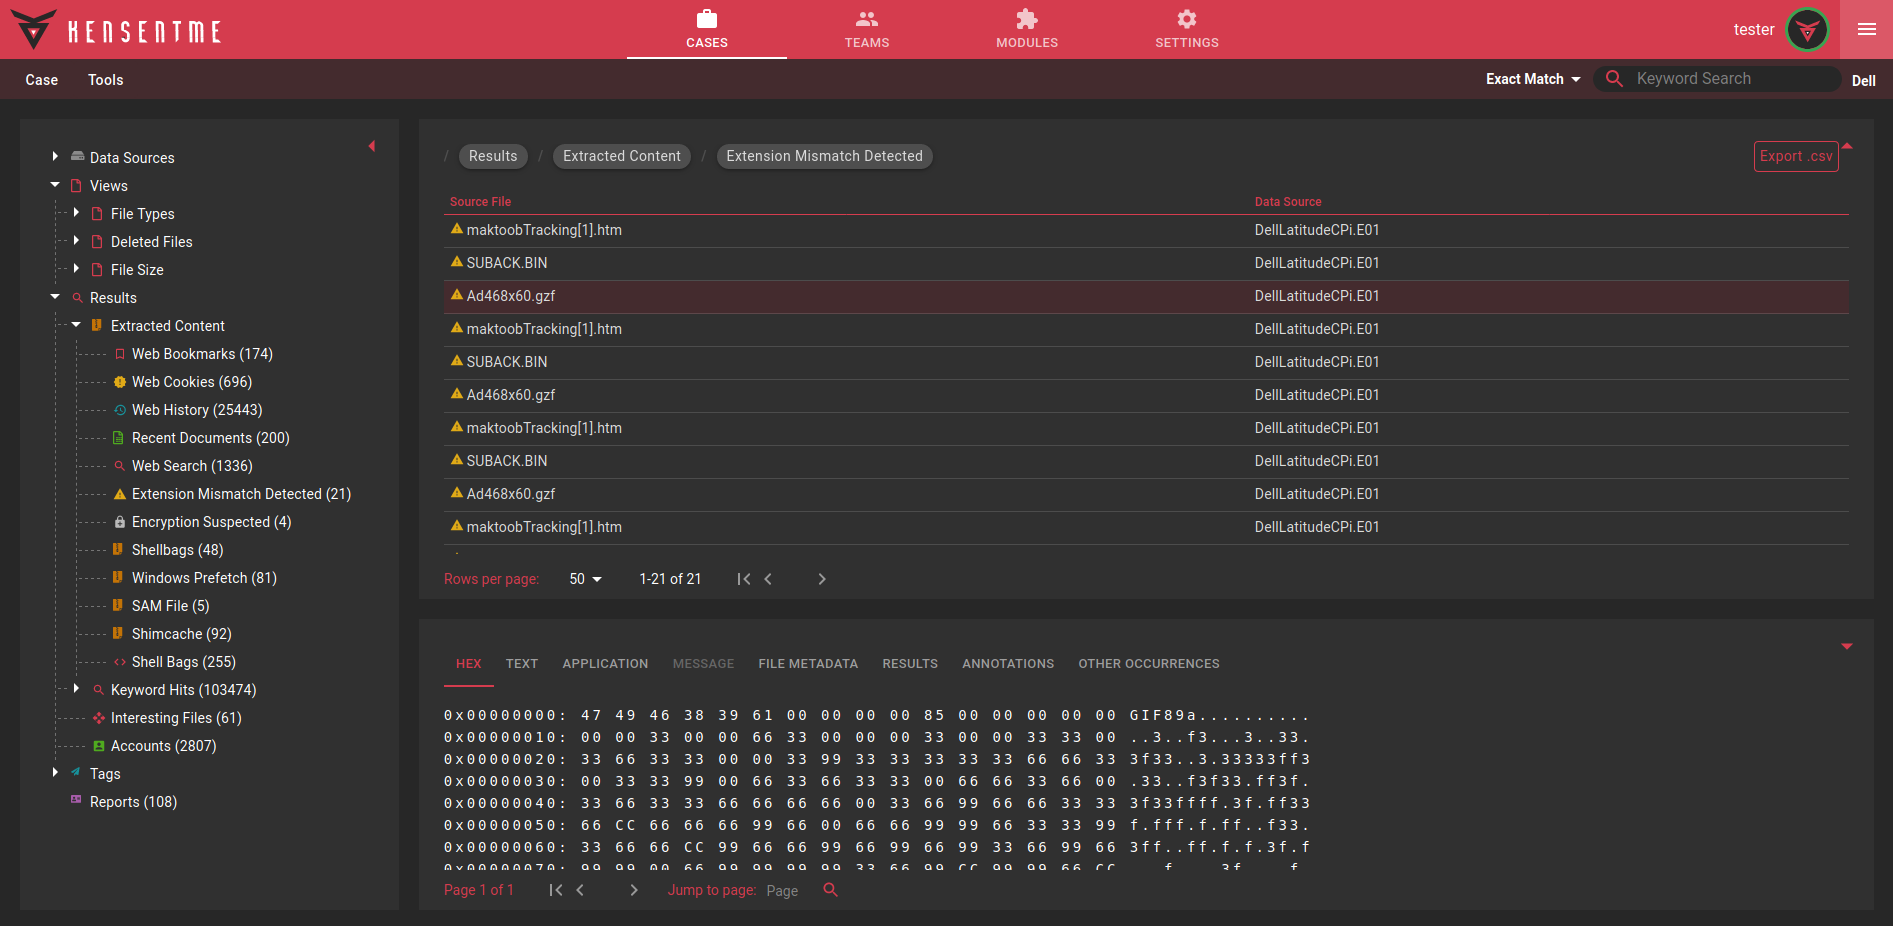
\includegraphics[width=1\linewidth]{imgs/data.png}
 \caption{Ingested Results Presentation}
 \label{fig:data}
\end{figure}

The content viewer can display different kinds of information depending on the type of item selected, these can be some of the following:
\begin{itemize}
 \item Text browser
 \item Media viewer
 \item Database browser
 \item Registry browser
 \item Key-value browser
 \item Table data viewer
\end{itemize}

The layout for the ingested results presentation, and for all the case related actions, was based on the original Autopsy layout, so that each container can be re-sized as
needed, allowing the user to focus on the information that is most important to him.

This development stage was one of the most intensive, as it required understanding Autopsy's data structure very well. The source code used here was rewritten almost completely, 
because of the way the user interface and the data structure in the original program and interconnected, resulting in the need to adapt and write custom queries to obtain the desired results, creating more than 
50 endpoints so that all the needed information could be supplied. As well as creating and adjusting all the UI elements to achieve an user experience similar to what Autopsy's users are used to.

\subsection{Tag Management}

Tagging content is a very important step in forensics investigations, as it allows the investigators to keep an organized list of important information.

Tagging was added to the platform in the form of a context menu, that is shown by selecting information from the table/thumbnail viewer.

Tags take the form of file or result tags, and the difference is that a result tag is specific to an artifact, while a file tag is related to the file itself.

Autopsy contains 10 different tag types by default, and more can be added, which can result in a very big number of tag types in use, which deteriorates the user experience.

Tag names are also shared between cases, so it seemed important to have more controll over the management of these tags, and the ability to delete tag types was added, even though it didn't exist in the original software.

Since each case contains it's own database, it's impossible to syncronize every case at once when a tag is deleted, so it was necessary to create a procedure to syncronize case tags when a case is opened.
 

\subsection{Data Sources}

Using the same credentials used to log-in to the platform, the user can also upload data source files into his folder located inside the server, using an FTP client like filezilla.
Then the user can browse these directories using the web interface and select a data source to add to the case, as can be seen in Figure \ref{fig:datasource}.

\begin{figure}[ht]
 \centering
 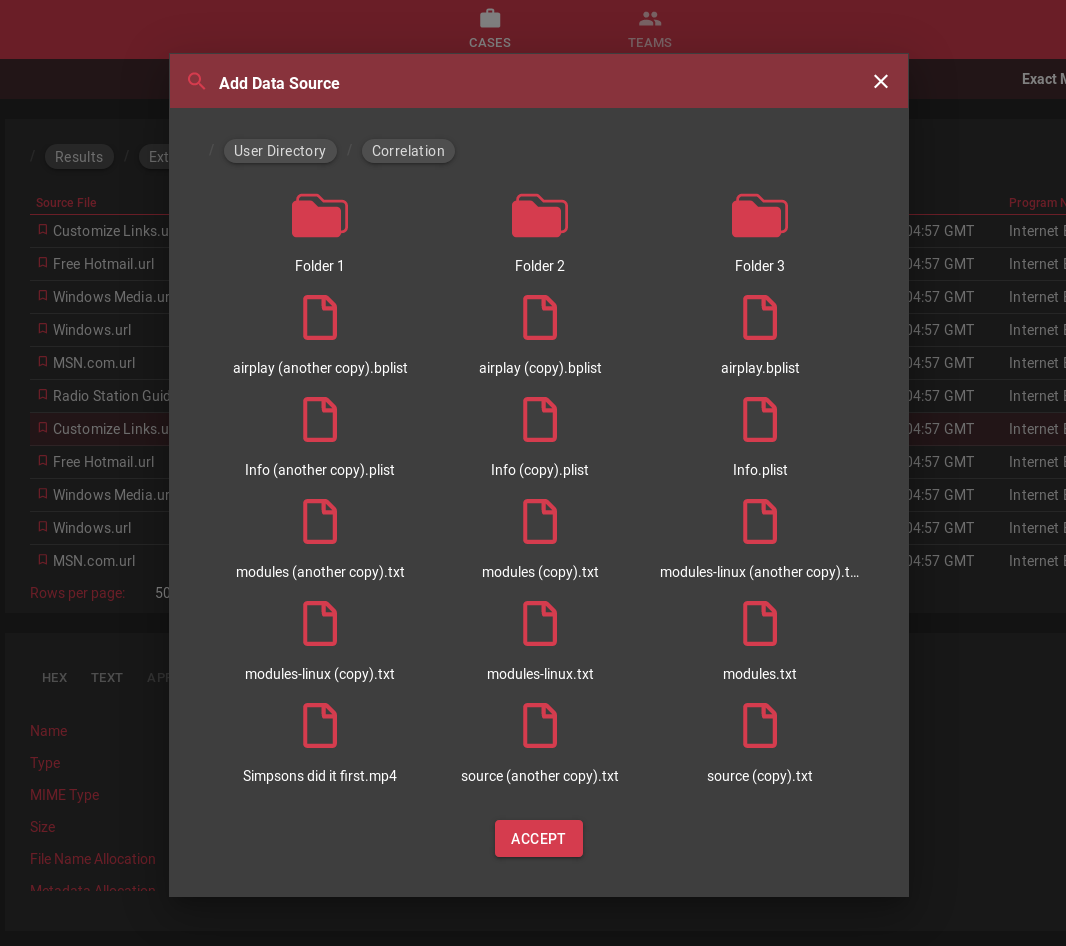
\includegraphics[width=0.75\linewidth]{imgs/data-sources.png}
 \caption{Data Source Selection}
 \label{fig:datasource}
\end{figure}

The procedure for adding a data source to a case was adapted from Autopsy's source code, and depends on the type of data source added, which can be one of the following:
\begin{itemize}
 \item Disk image
 \item Virtual machine
 \item Logical file collection
 \item Autopsy logical imager results
\end{itemize}

Local disk data sources were also an option provided by Autopsy but since the local disks the software has access to belong to a server, this feature is undesired.

When a data source is added to a case, it is processed and instances of abstract files and other entities are created, which allow the user to navigate the data source's contents as soon as it is processed.
Just navigating the data source contents isn't very useful, as the contents are in a raw state, showing mostly the file structure of the source, and not even categorizing files by mime types, so running data
ingestion modules is a critical step into allowing a deeper analysis of a data source, which is covered in the next section.

\subsection{Data Ingestion Modules}

Data ingestion modules can be either file ingest modules, which analyse each file contained in a data source, one by one,
or data source ingest modules, which run on specific components of a data source.

To run a collection of modules, the user selects which modules to run, and may also configure some parameters related to the modules, when the request is received by the server, the modules are started in a background thread.

When the modules are running the server communicates to each client through websockets, offering feedback on the progress of the modules, as can be seen in Figure \ref{fig:modules}.

\begin{figure}[ht]
 \centering
 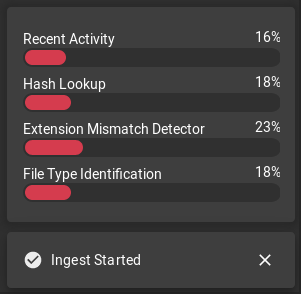
\includegraphics[width=0.55\linewidth]{imgs/modules.png}
 \caption{Ingest Modules Communication}
 \label{fig:modules}
\end{figure}

Originally it was intended to have the clients update their explorer as new information is ingested, but it would slow down the ingest progress considerably, so what was decided was that every client would refresh 
it's explorer every 30 seconds while ingests are running.

There were other measures taken into consideration to improve the performance of the ingest procedure, while also maintaining the user informed of it's progress, the server communicates a maximum of one file name per
second, and it also only communicates a module's progress when it advances at least one percentual point.

\subsection{Report Modules}

Report modules consist in generating a file or collection of files, to further process, filter, or present the results found in a case, it can take many shapes such as a text file, spreadsheets, HTML pages or even a portable case that can be imported into Autopsy.

Report modules have the ability to process existing data and generate results based on that, such as validating e-mail addresses or credit card numbers, 
which are found based on regular expressions by the keyword search module and may contain false positives.

The adaptation of the source code for report modules went pretty smoothly, with the exception that some modules require the user to provide a file when running the module, which resulted in the creation of a file repository within the server, for files to be used in this manner.

\subsection{Add-on Modules}

Autopsy supports third party modules in the form or netbeans module files (NBM), and in the form of python scripts, using the Jython language, which allows python code to run alongside classes defined in Java.

Since the developed platform doesn't support a java user interface, the procedure to install netbeans modules could not be implemented, as this feature is specific to netbeans applications. 
But most modules are made in the Jython language, and the addition of this modules was implemented as intended.

A user with a manager role can add new modules to the platform by uploading a zip archive containing the modules, the platform also allows management of the added modules, so that managers can enable, disabled and remove certain modules, as can be seen in Figure \ref{fig:settings}.

\begin{figure}[ht]
 \centering
 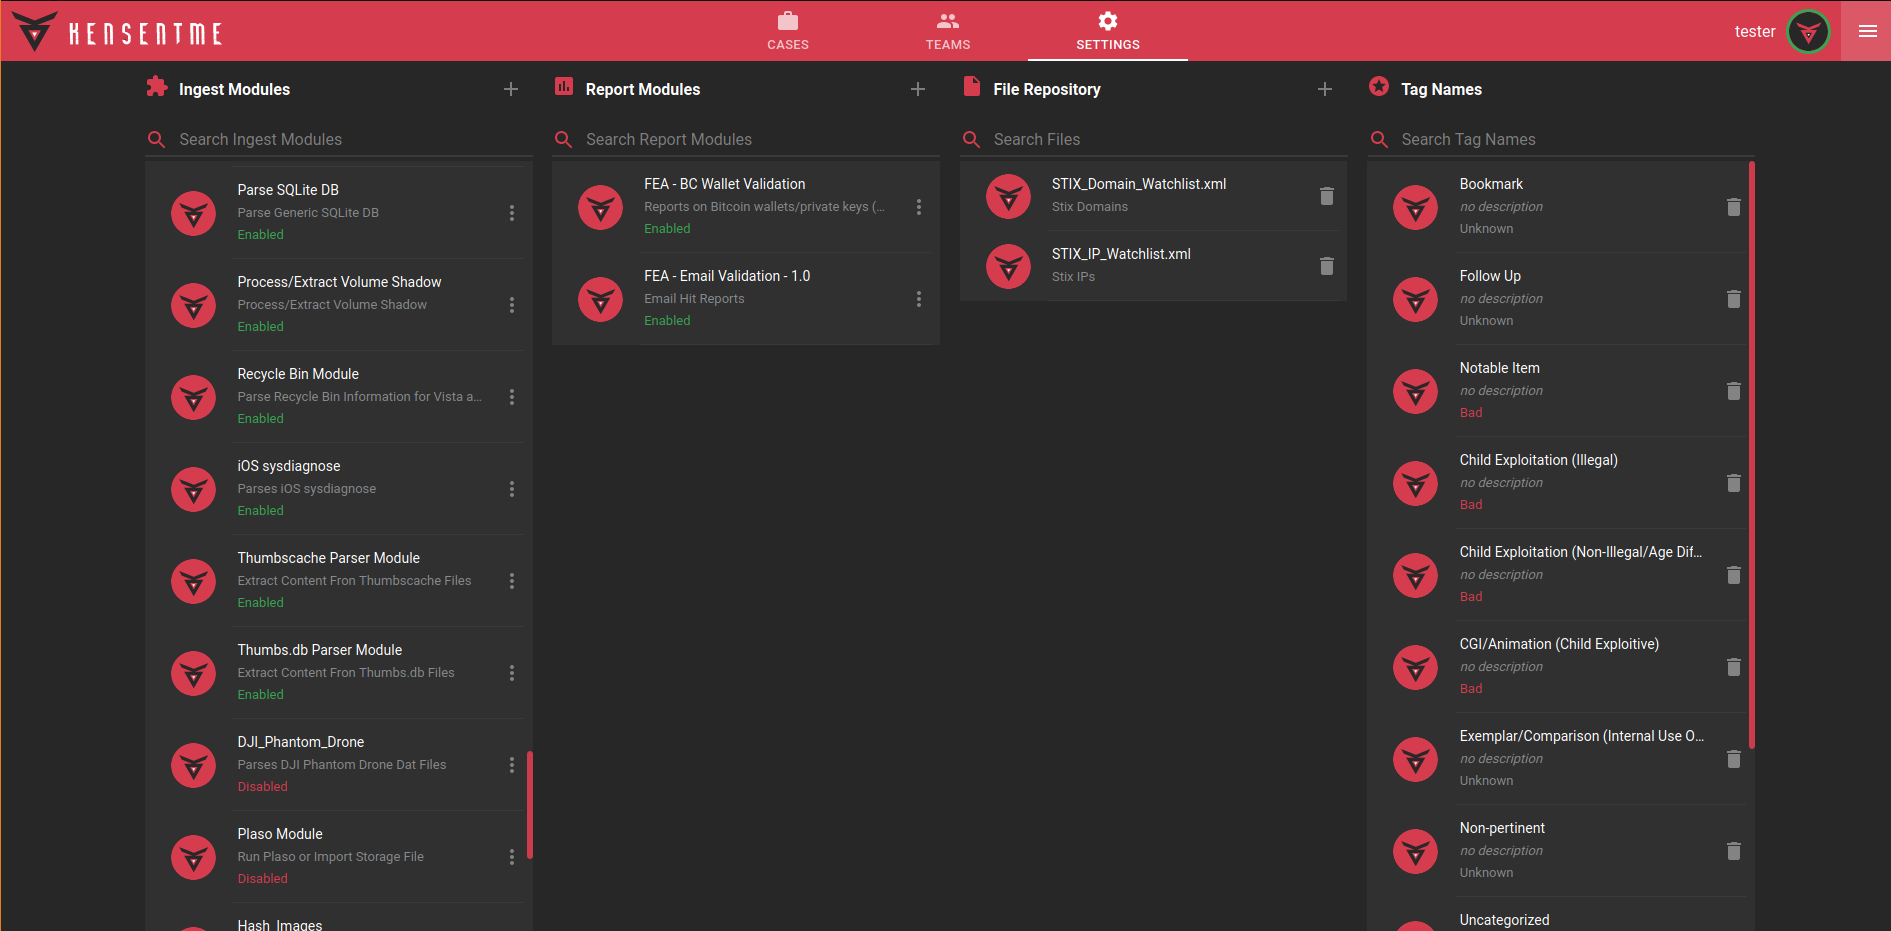
\includegraphics[width=1\linewidth]{imgs/settings.png}
 \caption{Add-on Modules Management}
 \label{fig:settings}
\end{figure}

Third party modules require that the original Autopsy source code is accessible in the original name space, which resulted in the seperation of the
developed and adapted code into two different name spaces, the original software's namespace which is org.sleuthkit.autopsy, and the company's namespace which is pt.voidsoftware.kensentme. 

This requirement of the original code can also mean that some modules which weren't tested may fail to run due to missing code, but a procedure to handle failure to run modules is implemented, 
and it informs the user about which modules are failing to run, allowing the user to disable the unsupported modules.

\subsection{Project Deployment}

A readme document was created, detailing each step required to setup the platform, which involves installing all the dependencies required, as well as compiling the developed code.

The setup was tested in multiple versions of Linux and with different versions of needed dependencies, resulting in a controlled step-by-step guide that can be followed in about 30 minutes that leads to a successful deployment of the complete platform.

\section{Critical Analysis and Proposed Improvements}

The development of the platform halted due to it being considered in a finished state, which means that all the objectives for the project were completed successfully.

Given that Autopsy is still in active development, it would be very important to keep following it's development, and complimenting this platform with new features and bug fixes which might come up in the future.

Besides accompanying Autopsy's improvements, it could also be interesting to further develop the platform to better serve the needs of it's users, which would require installations of the platform, and a feedback channel to better understand the user's needs.
